\section{Automata Web-Ebay}
\subsection{ Descripci\'on del programa}
\justify
El siguiente programa reconoce todas las palabras que contengan web o ebay,esto se realizar por medio de un automata finito determinista, podr\'a reconocer las palabras solo en textos en ingl\'es.\\
Consta de un modo autom\'atico y manual, ademas se podr\'a visualizar el diagrama del aut\'omata.\\
El programa guarda todas las palabras que encontr\'o y las guarda en un archivo de texto indicando el numero de fila y palabra en la que se encuentra.\\
\subsection{C\'odigo}
El c\'digo utilizado para la resoluci\'on del problema se muestra a continuaci\'on:\\

C\'odigo: webay.py
\lstset{language=Python, breaklines=true, basicstyle=\footnotesize}
\begin{lstlisting}[frame=single]
def automataWebay(caracter,estado,archivo):
	if(estado==0):
		estado=estadoCero(caracter,archivo)
	elif(estado==1):
		estado=estadoUno(caracter,archivo)
	elif(estado==2):
		estado=estadoDos(caracter,archivo)
	elif(estado==3):
		estado=estadoTres(caracter,archivo)
	elif(estado==4):
		estado=estadoCuatro(caracter,archivo)
	elif(estado==5):
		estado=estadoCinco(caracter,archivo)
	elif(estado==6):
		estado=estadoSeis(caracter,archivo)
	elif(estado==7):
		estado=estadoSiete(caracter,archivo)

	return estado

def estadoCero(caracter,archivo):
	if (caracter=='w'):
		archivo.write('q0--w-->q1\t')
		return 1
	elif (caracter=='e'):
		archivo.write('q0--e-->q4\t')
		return 4
	else:
		archivo.write('q0--%s-->q0\t' %caracter)
		return 0

def estadoUno(caracter,archivo):
	if(caracter=='w'):
		archivo.write('q1--w-->q1\t')
		return 1
	elif(caracter=='e'):
		archivo.write('q1--e-->q2\t')
		return 2
	else:
		archivo.write('q1--%s-->q0\t' % caracter)
		return 0

def estadoDos(caracter,archivo):
	if(caracter=='w'):
		archivo.write('q2--w-->q1\t')
		return 1
	elif(caracter=='e'):
		archivo.write('q2--e-->q4\t')
		return 4
	elif(caracter=='b'):
		archivo.write('q2--b-->q3\t')
		return 3
	else:
		archivo.write('q2--%s-->q0\t' % caracter)
		return 0

def estadoTres(caracter,archivo):
	if(caracter=='w'):
		archivo.write('q3--w-->q1\t')
		return 1
	elif(caracter=='e'):
		archivo.write('q3--e-->q4\t')
		return 4
	elif(caracter=='a'):
		archivo.write('q3--a-->q6\t')
		return 6
	else:
		archivo.write('q3--%s-->q0\t' % caracter)
		return 0

def estadoCuatro(caracter,archivo):
	if(caracter=='w'):
		archivo.write('q4--2-->q1\t')
		return 1
	elif(caracter=='e'):
		archivo.write('q4--e-->q4\t')
		return 4
	elif(caracter=='b'):
		archivo.write('q4--b-->q5\t')
		return 5
	else:
		archivo.write('q4--%s-->q0\t' % caracter)
		return 0

def estadoCinco(caracter,archivo):
	if(caracter=='w'):
		archivo.write('q5--w-->q1\t')
		return 1
	elif(caracter=='e'):
		archivo.write('q5--e-->q4\t')
		return 4
	elif(caracter=='a'):
		archivo.write('q5--a-->q6\t')
		return 6
	else:
		archivo.write('q5--%s-->q0\t' % caracter)
		return 0

def estadoSeis(caracter,archivo):
	if(caracter=='w'):
		archivo.write('q6--w-->q1\t')
		return 1
	elif(caracter=='e'):
		archivo.write('q6--e-->q4\t')
		return 4
	elif(caracter=='y'):
		archivo.write('q6--y-->q7\t')
		return 7
	else:
		archivo.write('q6--%s-->q0\t' % caracter)
		return 0

def estadoSiete(caracter,archivo):
	if(caracter=='w'):
		archivo.write('q7--w-->q1\t')
		return 1
	elif(caracter=='e'):
		archivo.write('q7--e-->q4\t')
		return 4
	else:
		archivo.write('q7--%s-->q0\t' % caracter)
		return 0

\end{lstlisting}
\vspace{1.5cm}
C\'odigo:main.py

\lstset{language=Python, breaklines=true, basicstyle=\footnotesize}
\begin{lstlisting}[frame=single]
import webay
import diagrama

def menu():
    try:
        opcion=input('\t\t-------------WEBAY------------\n1.-Modo manual\n2.-Leer texto\n3.-Diagrama\n4.-Salir\nElija una opcion: ')
        opcion=int(opcion)
    except:
        print('\nIntroduzca una opcion correcta\n')

    return opcion

def IniciarArchivo():
    archivo=open("Palabras.txt","w")
    archivo.close
    archivoH=open("Historia.txt","w")
    archivo.close

def AbrirArchivo():
    try:
        archivo=open("Palabras.txt","a")
    except:
        print("\nError al abrir el archivo")
        exit()
    return archivo

def AbrirHistoria():
    try:
        archivo=open("Historia.txt","a")
    except:
        print("\nError al abrir el archivo")
        exit()
    return archivo

def escribir(archivo,palabra_aux,no_palabra,no_fila):
    archivo.write("Palabra: "+palabra_aux+" Numero de palabra: "+str(no_palabra)+" Numero de fila: "+str(no_fila))
    archivo.write("\n")


def Evaluar(texto):
    archivo=AbrirArchivo()
    historia=AbrirHistoria()
    palabra_aux=''
    final=False
    estado=0
    no_palabra=1
    no_fila=1

    historia.write("\n\n\n\n")
    for caracter in texto:
        caracter=caracter.lower()
        estado=webay.automataWebay(caracter,estado,historia)
        if(estado==3 or estado==7):
            final=True
        if(caracter=='\n'):
            if(final):
                escribir(archivo,palabra_aux,no_palabra,no_fila)
                historia.write("\n")
                palabra_aux=''
                final=False
            else:
                palabra_aux=''
            no_palabra=1
            no_fila=no_fila+1
            continue
        if (caracter==' '):
            if(final):
                escribir(archivo,palabra_aux,no_palabra,no_fila)
                historia.write("\n")
                palabra_aux=''
                final=False
            else:
                palabra_aux=''
            no_palabra=no_palabra+1

            continue
        palabra_aux=palabra_aux+caracter
    if(final):
        no_palabra=no_palabra+1
        escribir(archivo,palabra_aux,no_palabra,no_fila)
        historia.write("\n")

    archivo.close
    historia.close
def leer_Archivo():
    try:
        archivo=open("archivo.txt","r")
        texto=str(archivo.read())
    except:
        print("\nError al abrir el archivo")
        exit()
    return texto

def main():
    IniciarArchivo()
    while True:
        eleccion=menu()
        if(eleccion==1):
            texto=input("Introduzca un pequenio texto: ")

            Evaluar(texto)
            print("Evaluacion terminada, cheque el archivo de texto")
            while True:
                reop=input("Desea regresar al menu\n1.-Si\n2.-No\nEleccion: ")
                if(reop=='1'):
                    break
                elif(reop=='2'):
                    exit()
                else:
                    continue
        elif(eleccion==2):
            texto=leer_Archivo()

            Evaluar(texto)
            print("Evaluacion terminada, cheque el archivo de texto")
            while True:
                reop=input("Desea regresar al menu\n1.-Si\n2.-No\nEleccion: ")
                if(reop=='1'):
                    break
                elif(reop=='2'):
                    exit()
                else:
                    continue
        elif(eleccion==3):
            diagrama.mostrarDiagrama()
            while True:
                reop=input("Desea regresar al menu\n1.-Si\n2.-No\nEleccion: ")
                if(reop=='1'):
                    break
                elif(reop=='2'):
                    exit()
                else:
                    continue
        elif(eleccion==4):
            exit()
        else:
            continue
main()


\end{lstlisting}
\vspace{1.5cm}
C\'odigo:diagrama.py

\lstset{language=Python, breaklines=true, basicstyle=\footnotesize}
\begin{lstlisting}[frame=single]
	rom tkinter import *

def mostrarDiagrama():
    ventana=Tk()
    ventana.geometry("900x650")
    ventana.resizable(width=False,height=False)
    ventana.title("Automata WEBAY")
    AreaDibujo=Canvas(ventana, width=900,height=650)
    AreaDibujo.pack()

    #Creacion de circulos de estados
    #inicio
    AreaDibujo.create_oval(50,275,150,375,fill="sky blue")

    #web
    AreaDibujo.create_oval(200,150,300,250,fill="sky blue")
    AreaDibujo.create_oval(400,150,500,250,fill="sky blue")
    AreaDibujo.create_oval(590,140,710,260,fill="white")
    AreaDibujo.create_oval(600,150,700,250,fill="sky blue")

    #ebay
    AreaDibujo.create_oval(200,400,300,500,fill="sky blue")
    AreaDibujo.create_oval(400,400,500,500,fill="sky blue")
    AreaDibujo.create_oval(600,400,700,500,fill="sky blue")
    AreaDibujo.create_oval(770,390,890,510,fill="white")
    AreaDibujo.create_oval(780,400,880,500,fill="sky blue")

    #creacion de lineas de transicion
    #inicio
    AreaDibujo.create_line(20,325,50,325)
    #web
    AreaDibujo.create_line(149,318,203,210)
    AreaDibujo.create_line(300,200,400,200)
    AreaDibujo.create_line(500,200,590,200)

    AreaDibujo.create_line(650,260,650,400)
    AreaDibujo.create_line(296,180,404,180)
    AreaDibujo.create_line(407,230,253,402)
    AreaDibujo.create_line(600,230,269,408)
    #ebay
    AreaDibujo.create_line(149,332,203,440)
    AreaDibujo.create_line(300,450,400,450)
    AreaDibujo.create_line(500,450,600,450)
    AreaDibujo.create_line(700,450,770,450)

    AreaDibujo.create_line(250,400,250,250)
    AreaDibujo.create_line(405,424,265,247)
    AreaDibujo.create_line(298,430,403,430)
    AreaDibujo.create_line(618,410,280,240)
    AreaDibujo.create_line(787,405,294,225)

    #creacion de arcos de transicion
    #inicio
    AreaDibujo.create_arc(60,240,110,305,start=-8,extent=219,style=ARC)
    #web
    AreaDibujo.create_arc(210,125,260,185,start=2,extent=210,style=ARC)
    AreaDibujo.create_arc(110,190,400,450,start=112,extent=50,style=ARC)
    AreaDibujo.create_arc(150,100,750,650,start=55,extent=72,style=ARC)
    AreaDibujo.create_arc(20,55,720,395,start=26,extent=181,style=ARC)
    AreaDibujo.create_arc(78,85,480,500,start=41,extent=137,style=ARC)

    #ebay
    AreaDibujo.create_arc(110,190,400,460,start=200,extent=48,style=ARC)
    AreaDibujo.create_arc(20,240,880,600,start=157,extent=173,style=ARC)
    AreaDibujo.create_arc(200,385,890,550,start=45,extent=95,style=ARC)
    AreaDibujo.create_arc(70,85,770,571,start=189,extent=128,style=ARC)
    AreaDibujo.create_arc(90,85,560,520,start=199,extent=98,style=ARC)
    AreaDibujo.create_arc(250,390,625,550,start=200,extent=146,style=ARC)
    AreaDibujo.create_arc(208,442,285,530,start=172,extent=185,style=ARC)


    #creacion de circulos de indicacion
    #inicio
    AreaDibujo.create_oval(47,322,53,328,fill="black")
    #web
    AreaDibujo.create_oval(52,296,58,302,fill="black")
    AreaDibujo.create_oval(61,285,67,291,fill="black")
    AreaDibujo.create_oval(76,278,82,284,fill="black")
    AreaDibujo.create_oval(115,275,121,281,fill="black")

    AreaDibujo.create_oval(198,209,204,215,fill="black")
    AreaDibujo.create_oval(397,197,403,203,fill="black")
    AreaDibujo.create_oval(587,197,593,203,fill="black")
    AreaDibujo.create_oval(210,166,216,172,fill="black")

    AreaDibujo.create_oval(293,177,299,183,fill="black")
    AreaDibujo.create_oval(269,152,275,158,fill="black")
    AreaDibujo.create_oval(647,397,653,403,fill="black")

    AreaDibujo.create_oval(253,397,259,403,fill="black")
    AreaDibujo.create_oval(268,403,274,409,fill="black")
    #ebay
    AreaDibujo.create_oval(53,346,59,352,fill="black")
    AreaDibujo.create_oval(72,365,78,371,fill="black")
    AreaDibujo.create_oval(102,372,108,378,fill="black")
    AreaDibujo.create_oval(117,368,123,374,fill="black")

    AreaDibujo.create_oval(199,436,205,442,fill="black")
    AreaDibujo.create_oval(206,476,212,482,fill="black")
    AreaDibujo.create_oval(297,447,303,453,fill="black")

    AreaDibujo.create_oval(259,495,265,501,fill="black")
    AreaDibujo.create_oval(278,411,284,417,fill="black")
    AreaDibujo.create_oval(247,247,253,253,fill="black")
    AreaDibujo.create_oval(399,427,405,433,fill="black")

    AreaDibujo.create_oval(263,245,269,251,fill="black")
    AreaDibujo.create_oval(597,447,603,453,fill="black")

    AreaDibujo.create_oval(276,238,282,244,fill="black")
    AreaDibujo.create_oval(768,447,774,453,fill="black")

    AreaDibujo.create_oval(292,223,298,229,fill="black")

    #etiquetas
    #inicio
    inicio=Label(ventana,text="inicio",font="Verdana 6").place(x=20,y=305)
    #estados
    q0=Label(ventana,text="q0",font="Verdana 10",background="sky blue").place(x=90,y=317)
    q1=Label(ventana,text="q1",font="Verdana 10",background="sky blue").place(x=240,y=190)
    q2=Label(ventana,text="q2",font="Verdana 10",background="sky blue").place(x=440,y=190)
    q3=Label(ventana,text="q3",font="Verdana 10",background="sky blue").place(x=640,y=190)
    q4=Label(ventana,text="q4",font="Verdana 10",background="sky blue").place(x=240,y=440)
    q5=Label(ventana,text="q5",font="Verdana 10",background="sky blue").place(x=440,y=440)
    q6=Label(ventana,text="q6",font="Verdana 10",background="sky blue").place(x=640,y=440)
    q7=Label(ventana,text="q7",font="Verdana 10",background="sky blue").place(x=820,y=440)
    #web
    w1=Label(ventana,text="w",font="Verdana 7").place(x=165,y=285)
    w2=Label(ventana,text="no es w,e",font="Verdana 7").place(x=125,y=212)
    w3=Label(ventana,text="e",font="Verdana 7").place(x=165,y=345)
    w4=Label(ventana,text="w",font="Verdana 7").place(x=390,y=160)
    w5=Label(ventana,text="e",font="Verdana 7").place(x=310,y=190)
    w6=Label(ventana,text="w",font="Verdana 7").place(x=220,y=120)
    w7=Label(ventana,text="w",font="Verdana 7").place(x=455,y=105)

    w8=Label(ventana,text="b",font="Verdana 7").place(x=510,y=190)
    w9=Label(ventana,text="no es w,e,a",font="Verdana 7").place(x=455,y=40)
    w10=Label(ventana,text="no es w,e,b",font="Verdana 7").place(x=245,y=95)
    w11=Label(ventana,text="e",font="Verdana 7").place(x=390,y=215)
    w12=Label(ventana,text="e",font="Verdana 7").place(x=580,y=215)
    w13=Label(ventana,text="a",font="Verdana 7").place(x=660,y=270)
    #ebay
    e1=Label(ventana,text="no es w,e,b",font="Verdana 6").place(x=120,y=385)
    e2=Label(ventana,text="e",font="Verdana 7").place(x=263,y=525)
    e3=Label(ventana,text="b",font="Verdana 7").place(x=310,y=412)
    e4=Label(ventana,text="e",font="Verdana 7").place(x=380,y=455)
    e5=Label(ventana,text="a",font="Verdana 7").place(x=510,y=430)
    e6=Label(ventana,text="y",font="Verdana 7").place(x=710,y=430)

    e7=Label(ventana,text="e",font="Verdana 7").place(x=710,y=400)
    e8=Label(ventana,text="e",font="Verdana 7").place(x=580,y=476)
    e9=Label(ventana,text="w",font="Verdana 7").place(x=710,y=355)
    e10=Label(ventana,text="w",font="Verdana 7").place(x=550,y=355)
    e11=Label(ventana,text="w",font="Verdana 7").place(x=370,y=360)
    e12=Label(ventana,text="w",font="Verdana 7").place(x=230,y=370)

    e13=Label(ventana,text="no es w,e",font="Verdana 7").place(x=450,y=605)
    e14=Label(ventana,text="no es w,e,a",font="Verdana 7").place(x=425,y=505)
    e15=Label(ventana,text="no es e,y,w",font="Verdana 7").place(x=470,y=570)
    e16=Label(ventana,text="no es w,e",font="Verdana 6").place(x=35,y=220)




    ventana.mainloop()	
	
\end{lstlisting}

\newpage

\subsection{Pruebas}
A continuaci\'on se mostraran algunas im\'agenes capturadas al momento de ejecutar el programa, dichas im\'agenes mostraran los resultados obtenidos.\\
\vspace{1.0cm}
Para el modo manual:\\
\begin{figure}[H]
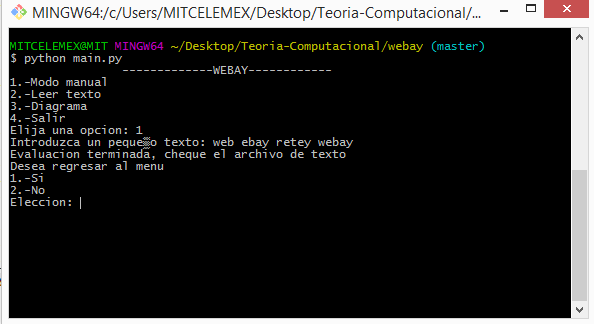
\includegraphics[width=\textwidth, height=7cm]{ModoManualWebay.png}
\label{fig:manual_webay}
\caption{Palabras de prueba: web ebay retey webay}
\end{figure}

\begin{figure}[H]
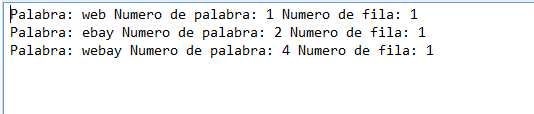
\includegraphics[width=\textwidth, height=7cm]{ArchivoWebay.png}
\label{fig:manualtexto_alfabeto}
\caption{Salida del archivo de palabras encontradas}
\end{figure}

\begin{figure}[H]
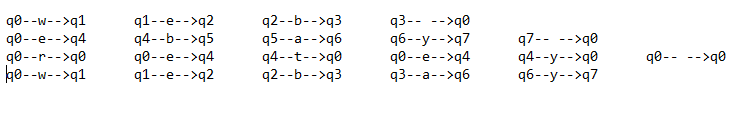
\includegraphics[width=\textwidth, height=7cm]{HistoriaWebay.png}
\label{fig:manualnuevoconteo_alfabeto}
\caption{Historia de la evaluaci\'on del aut\'omata}
\end{figure}

Para el modo de lectura de un archivo:\\
\begin{figure}[H]
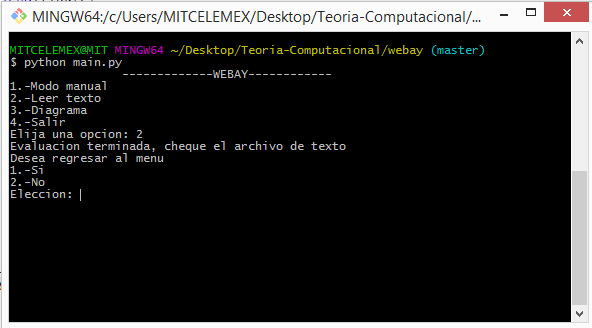
\includegraphics[width=\textwidth, height=7cm]{ModoAutomaticoWebay.png}
\label{fig:auto_alfabeto}
\caption{Lectura de un texto con palabras WEB}
\end{figure}

\begin{figure}[H]
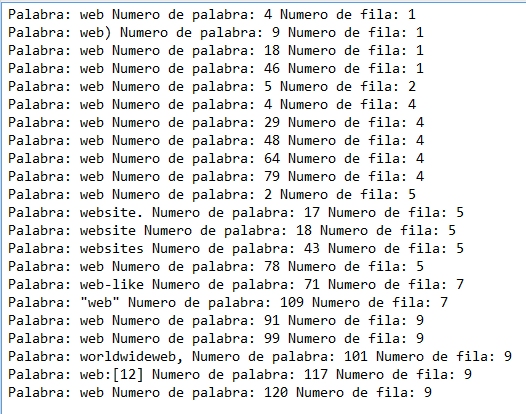
\includegraphics[width=\textwidth, height=7cm]{ArchivoTextoWebay.png}
\label{fig:autotexto_alfabeto}
\caption{Palabras encontradas del texto}
\end{figure}

\begin{figure}[H]
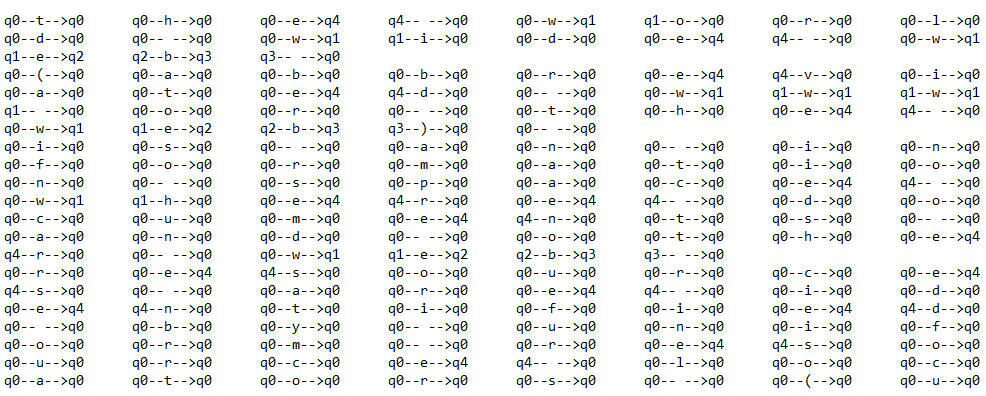
\includegraphics[width=\textwidth, height=7cm]{HistoriaWebayA.png}
\label{fig:manualnuevoconteo_alfabeto}
\caption{Historia de la evaluaci\'on del aut\'omata}
\end{figure}

\begin{figure}[H]
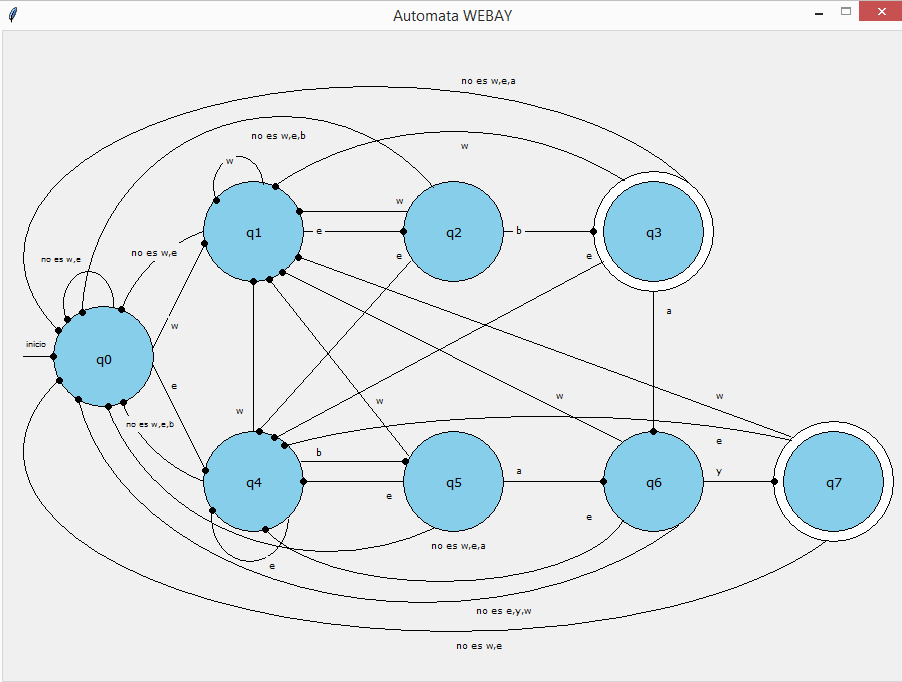
\includegraphics[width=\textwidth, height=7cm]{DiagramaWebay.png}
\label{fig:DiagramaWebay}
\caption{Diagrama del aut\'omata}
\end{figure}

\newpage

